% !Mode:: "TeX:UTF-8"

\chapter{绪论}

\section{课题背景及意义}

随着智能化技术的快速进步，城市公园、景区、社区等封闭场景中的用于休闲代步工具需求日益增多。人们对一种能够随时召唤、自动行驶且乘坐舒适的低速、稳定、安全的交通工具需求尤为突出。然而，传统的交通工具在这些环境中难以兼顾灵活性、安全性和便捷性，无法充分满足休闲和安全的双重需求。在这种背景下，两轮平衡车以其结构紧凑、操控灵活的特点，成为公园中代步工具的理想选择。如何保证两轮平衡车在这些复杂场景中的稳定行驶并感知周围环境，已成为该领域的重要研究课题。

为实现灵活、安全且舒适的目标，两轮平衡车的结构设计至关重要。当前常见的两轮平衡车结构包括以车轮控制为核心的Segway式平衡车、由Segway演变而来的可变结构两轮车、通过改变重心控制的平衡车，以及采用力矩控制陀螺CMG（Control Moment Gyroscope）的倒立摆机器人等。Segway式平衡车结构紧凑，操控性好且技术成熟，但其平衡依赖车体移动，限制了静态场景的应用，且在较大外部扭矩或冲击下，电机调整能力不足；可变结构平衡车提高了灵活性，但在稳定性方面仍存在较大问题；CMG倒立摆机器人能够更精确地控制姿态，但其存在能耗高、噪声等问题。这些现有结构难以在灵活性、安全性和乘坐舒适性之间找到最佳平衡，亟需进一步研究以探索更加优化的解决方案。

为了确保两轮平衡车在复杂环境中精确感知障碍物并及时反应，环境感知技术至关重要。目前主流技术包括激光雷达、毫米波雷达、ToF（Time to Fly）红外光传感器和双目相机。激光雷达虽然精度高，但成本较为昂贵；毫米波雷达具有较强的抗干扰能力，尤其在恶劣天气条件下表现出色，但其精度和分辨率在复杂环境中有所不足。ToF易受到光线、天气等环境因素影响。在综合考虑成本、精度和抗干扰能力后，双目相机凭借视差获取深度信息，逐渐展现出其高性价比和环境适应性，且结合深度学习可以显著提高障碍物检测的精度和鲁棒性，成为应对复杂环境感知需求的有效研究方向。

本课题将对两轮平衡车的部分技术开展研究，包括两轮平衡车的总体设计、基于双目视觉和深度学习的障碍物感知和感知与系统的设计和开发。双轮平衡车能够负载100kg，最高时速10km/h；完成对于双目视觉感知模块的研究，具备感知尺寸大于50x50x50cm的障碍物的能力，最终能在15m内能够识别典型障碍物。

\section{国内外研究现状}

\subsection{两轮平衡车结构的国内外研究现状}

两轮平衡车的结构设计是影响其性能的关键因素。合理的机械布局和平衡方式能够提升车辆的稳定性和操控性，因此，如何优化两轮平衡车的结构成为研究的重点方向。

1912年，英国谢洛夫斯基发明了基于力矩陀螺的两轮车，该车使用一个陀螺来保持车辆的平衡。1988年，俄国本资诺斯等人在该基础上发明了一款在运动过程中保持平衡的自行车机器人，该机器人上安置了一对控制力矩陀螺来产生力矩平衡车身稳定。该实验表明了力矩陀螺效应对平衡自行车机器人的作用。

最早成型的两轮平衡车，即Segway平衡车，是在1985年日本电通大学的山腾一雄教授构思的，由于当时能提供的硬件技术和控制理论有限，最终的研发结果不是很理想。21世纪开始，Segway平衡车在国外开始商业化，2006年，美国的Segway二代在市场上研究取得巨大成功。

1996年，Naoji Shiroma等人设计了一款两轮车如图~\ref{fig:NaojiShiroma两轮车}所示，Naoji Shiroma建立了系统的模型，并通过系统稳定性特征方程求解特征根的方式完成了两轮车机器人提升重物的实验。

\begin{figure}[!htbp]
  \centering
  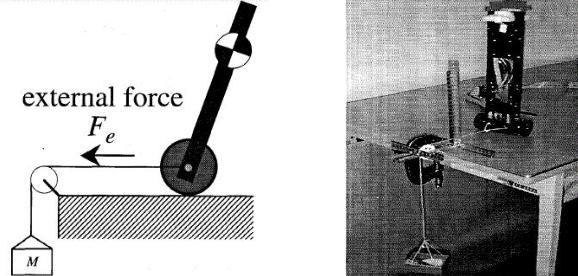
\includegraphics[width=0.85\textwidth]{figures/chapter01/NaojiShiroma等人设计的两轮车.png}
  \caption{Naoji Shiroma等人设计的两轮车}
  \label{fig:NaojiShiroma两轮车}
\end{figure}

2005年，哈尔滨工业大学王晓宇博士等人制作了两轮直立自平衡机器人，如图~\ref{fig:王晓宇HitBot两轮机器人}所示，利用拉格朗日法建立了机器人的动力学方程，并设计了自适应控制器来实现机器人的动态平衡。同时，他们还采用了Levenberg-.Marquardt最小二乘迭代法建立传感器的误差模型，以及采用了两级分散式异构卡尔曼滤波算法来实现机器人的组合导航。此外，王晓宇博士等人还分析比较了几种可以减少两轮机器人能量消耗的方法，这些方法包括使用摩擦力补偿器、使用能量回收技术以及改变机器人的行驶策略等。

\begin{figure}[!htbp]
  \centering
  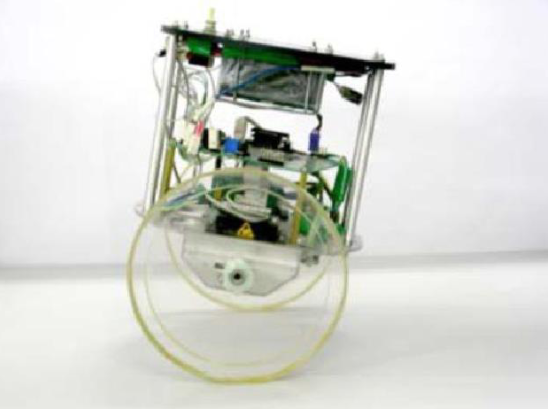
\includegraphics[width=0.85\textwidth]{figures/chapter01/王晓宇设计的HitBot两轮机器人.png}
  \caption{王晓宇设计的HitBot两轮机器人}
  \label{fig:王晓宇HitBot两轮机器人}
\end{figure}

2009年，北京工业大学的阮晓钢、赵建伟研究了一种直立式的自平衡辆车机器人，并在控制中引入了PWM（Pulse-width modulation）直流伺服控制系统。他们通过Matlab设计了LQR（Linear Quadratic Regulator）平衡控制器，接着进行了数值仿真和物理实验，实验结果表明两轮车机器人可以完成直立平衡行走。

2005年，日本千叶大学研究学者Minh-Quan DAO和Kang-Zhi LIU在独轮车的基础上加制了一对力矩陀螺，力矩陀螺结构为上下分布，该两对力矩陀螺以相反的速度高速运转，通过相反的陀螺进动来产生陀螺力矩来平衡车辆机器人的侧向平衡，通过车轮的驱动来实现车辆机器人的俯仰平衡，该研究团队选用拉格朗日方法建模，采用了LQR、H、常数限H等控制方法，最后实验实现了机器人姿态控制和纵向轨迹控制。模型如图~\ref{fig:力矩陀螺独轮车}所示。

\begin{figure}[!htbp]
  \centering
  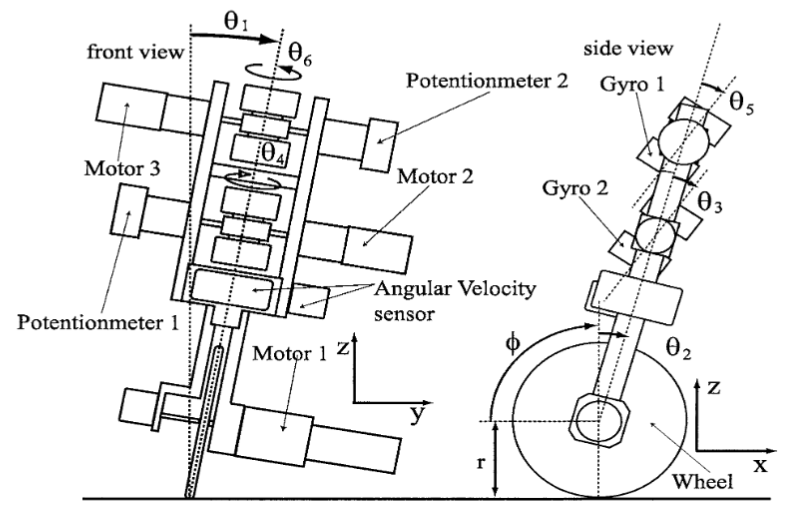
\includegraphics[width=0.85\textwidth]{figures/chapter01/力矩陀螺的独轮车.png}
  \caption{力矩陀螺的独轮车}
  \label{fig:力矩陀螺独轮车}
\end{figure}

2009年，北京邮电大学的刘大亮、孙汉旭和贾庆轩共同研发了一种具备动态平衡和载人行走能力的两轮机器人。该机器人由两个独立驱动的同轴车轮、可转动的厢体和固定在厢体上的操纵杆组成。通过操纵杆的倾斜，机器人能够实现前进、后退和转向动作，同时保持动态平衡。该机器人的设计注重安全性，允许在出现异常时，操作者能够安全地跳离车体，避免被操作机构绊倒。

2011年，北京邮电大学的孟祥珺等设计了一种变结构两轮车机器人的实体样机，如图~\ref{fig:变结构两轮车样机}所示，该两轮车机器人通过转动车轮角度，来改变机器人模式，车把转动至并列形式可形成segway模式，也可以如图中示意的车轮转动呈一字排布的自行车模式。

\begin{figure}[!htbp]
  \centering
  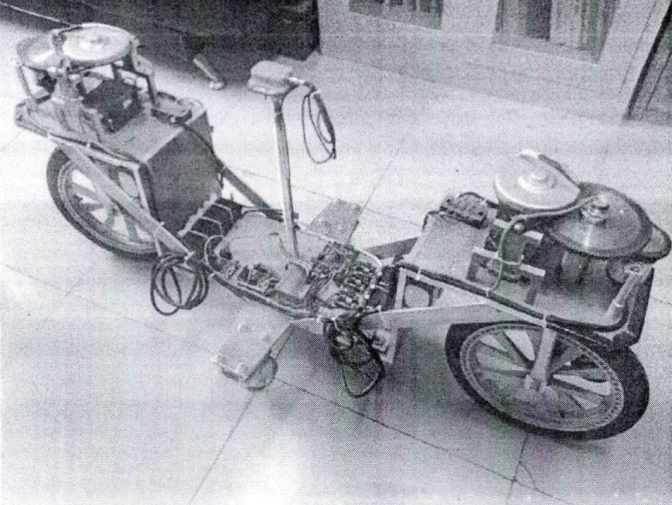
\includegraphics[width=0.85\textwidth]{figures/chapter01/变结构两轮车机器人样机.png}
  \caption{变结构两轮车机器人样机}
  \label{fig:变结构两轮车样机}
\end{figure}

2012年，美国加州的Lit Motor公司推出了一款两轮电动摩托车概念产品，代号为C-1，如图~\ref{fig:LitMotor内部结构}所示。该车拥有全封闭的汽车外观，车的底盘部分相比普通摩托车加装了一对高速旋转的力矩陀螺，如图~\ref{fig:LitMotor内部结构}所示，使得该款摩托车在停止，行驶和转弯时候能够保持车身稳定不倒。

\begin{figure}[!htbp]
  \centering
  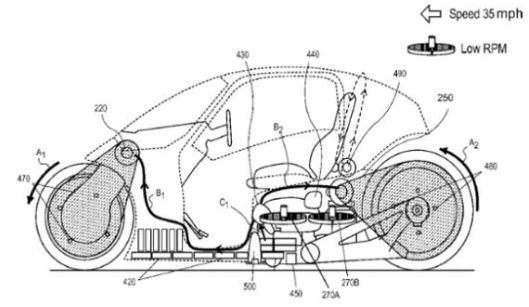
\includegraphics[width=0.85\textwidth]{figures/chapter01/美国加州的LitMotor公司推出的LitMotor内部结构图.png}
  \caption{美国加州的Lit Motor公司推出的Lit Motor内部结构图}
  \label{fig:LitMotor内部结构}
\end{figure}

2015年，戴福全在北京理工大学的研究中取得了重要进展，他设计并研制了一款具有多自由度和可变重心的两轮机器人如图~\ref{fig:可变重心两轮机器人}所示，这一创新性的设计在机器人领域引起了广泛的关注。这款机器人采用了卡尔曼滤波和摩擦补偿等技术来实现滑模控制，进一步提高了机器人的控制性能。

\begin{figure}[!htbp]
  \centering
  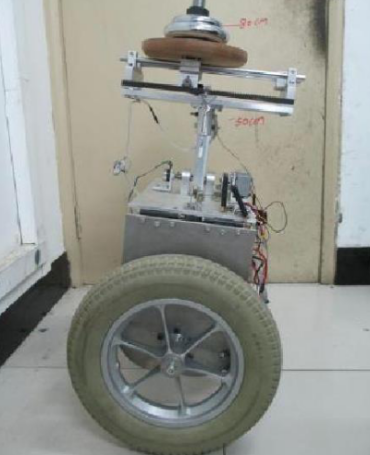
\includegraphics[width=0.85\textwidth]{figures/chapter01/可变重心的两轮机器人.png}
  \caption{可变重心的两轮机器人}
  \label{fig:可变重心两轮机器人}
\end{figure}

20l6年泰国亚洲理工学院的Surachat Chantarachit、ManukidParnichkun等人设计了一款具有力矩陀螺机构的独轮车机器人，如图~\ref{fig:亚洲理工独轮车机器人}所示，该独轮车采用的是左右分布放置两个力矩陀螺的方案，同样的利用控制力矩陀螺的原理控制独轮车的侧向平衡，车轮驱动力矩控制机器人的俯仰平衡。

\begin{figure}[!htbp]
  \centering
  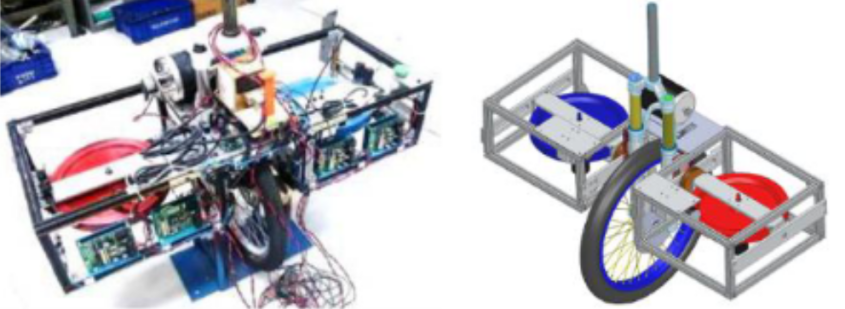
\includegraphics[width=0.85\textwidth]{figures/chapter01/亚洲理工学院设计的独轮车机器人.png}
  \caption{亚洲理工学院设计的独轮车机器人}
  \label{fig:亚洲理工独轮车机器人}
\end{figure}

2018年，桂林电子科技大学的黄用华设计了一种变结构两轮车机器人，如图~\ref{fig:黄用华两轮车机器人}所示。机器人采用Chaplygin建立动力学模型，使用部分反馈线性化控制器，然后进行了不同角度固定车把定车实验，行进过程中车轮角度切换等实验。

\begin{figure}[!htbp]
  \centering
  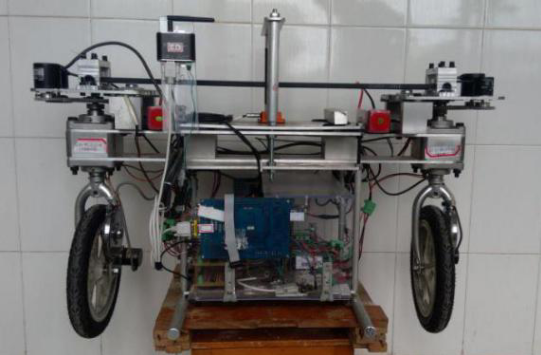
\includegraphics[width=0.85\textwidth]{figures/chapter01/黄用华设计的两轮车机器人.png}
  \caption{黄用华设计的两轮车机器人}
  \label{fig:黄用华两轮车机器人}
\end{figure}

2019年Kunitoshi Tanaka和Sumito Nagasawa提出了一种利用CMG来获得所需恢复力的倒立摆机器人如图~\ref{fig:KunitoshiTanakaCMG倒立摆机器人}所示。CMG的效果降低了机器人倾倒的速度，这意味着它可以在不移动的情况下保持平衡。研究成功展示了采用CMG的倒立摆机器人可以将姿态稳定性控制和轨迹跟踪控制分离。

\begin{figure}[!htbp]
  \centering
  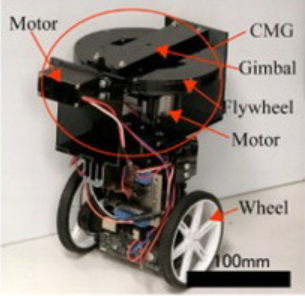
\includegraphics[width=0.85\textwidth]{figures/chapter01/KunitoshiTanaka设计的基于CMG的倒立摆机器人.png}
  \caption{Kunitoshi Tanaka设计的基于CMG的倒立摆机器人}
  \label{fig:KunitoshiTanakaCMG倒立摆机器人}
\end{figure}

2020年，苏黎世联邦理工学院设计和开发的一款高度先进的腿式机器人Ascento。如图~\ref{fig:Ascento轮腿机器人}所示。该机器人能够行走、奔跑、跳跃，甚至行杂技动作。Ascento的设计灵感来自猫和灵长类动物等动物的解剖结构和运动。它有四条单独驱动的腿，使其能够以极大的敏捷性和稳定性在广泛的方向上移动。机器人的身体也非常灵活，使其能够扭曲和适应不同的地形和障碍物。Ascento设计的关键创新之一是使用节能的电力驱动系统，该系统利用电机和弹簧的独特组合来实现高效率和动态性能。这使得机器人可以长时间运行，而无需频繁充电或维护。

\begin{figure}[!htbp]
  \centering
  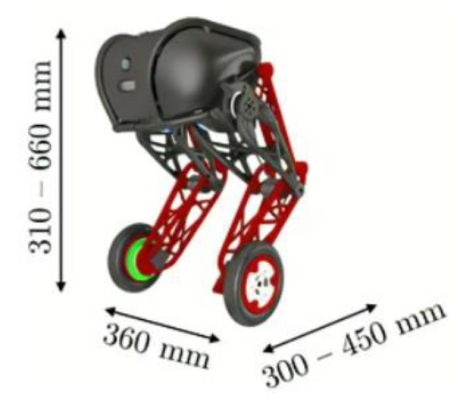
\includegraphics[width=0.85\textwidth]{figures/chapter01/Ascento轮腿机器人.png}
  \caption{Ascento轮腿机器人}
  \label{fig:Ascento轮腿机器人}
\end{figure}

2023年，Ahmed Ami和Moustafa A. Fouz等人设计了一种装备剪刀对控制力矩陀螺的两轮倒立摆机器人，旨在通过轮子驱动力矩实现稳定倾斜角度。研究将数学模型分为稳定性和运动性两个子系统，其中稳定性子系统在零状态下线性化以获取状态空间模型，并采用线性二次调节器（LQR）优化全状态反馈增益以实现平衡状态。运动子系统则独立于稳定性子系统进行力矩控制。

2024年，Gökhan Çetin通过拉格朗日方程推导了CMG机器人的运动方程，并使用Matlab模拟了未受控陀螺的平衡性能，以确定机电系统设计的期望配置。然后，将LQR应用于选定的CMG配置，并在RecurDyn的仿真中进行比较。LQR控制器被用来防止在武器后坐力作用下双CMG的振荡运动。仿真结果表明，采用LQR控制器的陀螺两轮机器人在静态下具有出色的性能，实现了显著的平衡改善。

\begin{figure}[!htbp]
  \centering
  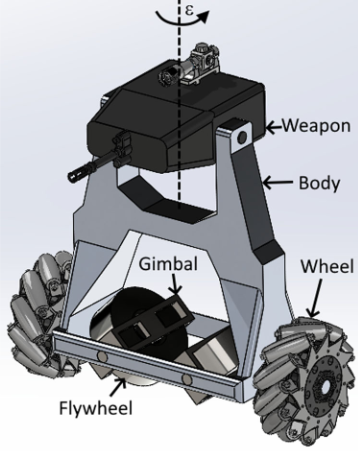
\includegraphics[width=0.85\textwidth]{figures/chapter01/GokhanCetin设计的装备有武器系统的力矩控制陀螺两轮机器人.png}
  \caption{Gökhan Çetin设计的装备有武器系统的力矩控制陀螺两轮机器人}
  \label{fig:GokhanCetin武器系统陀螺两轮机器人}
\end{figure}

\subsection{基于双目视觉的障碍物感知国内外研究现状}

双轮平衡车的安全性依赖于准确的障碍物感知。随着自动驾驶技术的发展，研究基于双目视觉的障碍物感知技术对于提升平衡车的安全性尤为重要。

2016年，Jonathan David Estilo等人实现了一种用于自动驾驶车辆的模块化障碍物检测系统，该系统结合了双目立体视觉和运动场技术。双目立体视觉算法使用立体块匹配算法来计算空间相邻图像之间的视差。运动场算法则利用FAST角点检测器和ORBsss关键点描述符来计算时间相邻图像的速度向量。实验结果表明，该模块能够成功检测到特征丰富的障碍物如车辆和行人，但在检测无特征障碍物时未能成功。

\begin{figure}[!htbp]
  \centering
  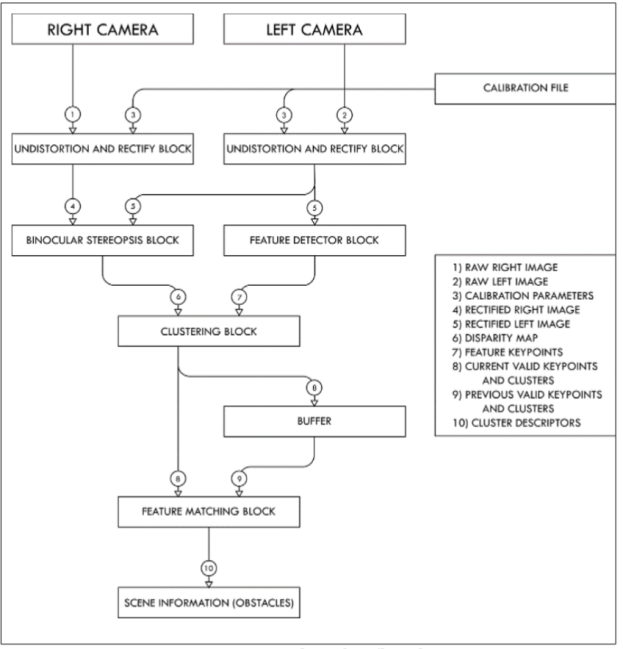
\includegraphics[width=0.85\textwidth]{figures/chapter01/检测演算流程.png}
  \caption{检测演算流程}
  \label{fig:检测演算流程}
\end{figure}

2018年，胡颖等人设计提出了一种基于卷积神经网络（CNN）的改进方法。该方法首先设计了孪生CNN来计算立体图像对的视差图，以提高匹配精度。接着，引入了一种道路直线自适应阈值提取算法，该算法能够精确地从视差图中提取出道路直线。最后，采用光栅扫描法对每个像素点进行障碍物检测，生成障碍检测图。实验结果证实了该方法在生成精确视差图、提取道路直线和精确识别路面障碍物方面的有效性，显著提升了检测的召回率和准确率。

\begin{figure}[!htbp]
  \centering
  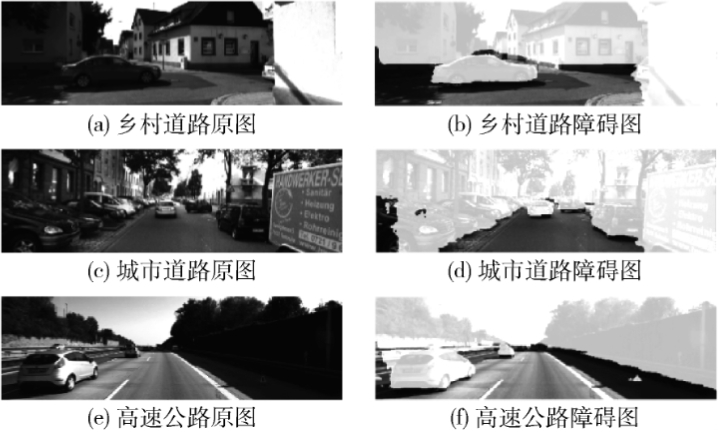
\includegraphics[width=0.85\textwidth]{figures/chapter01/光栅扫描法分割障碍物与道路.png}
  \caption{光栅扫描法分割障碍物与道路}
  \label{fig:光栅扫描分割障碍物与道路}
\end{figure}

2018年，清华大学的彭秋辰，宋亦旭提出一种基于MskR-CNN模型的双目视觉的物体识别和定位方法。该方法利用MskR-CNN处理双目图像，对每张图像进行物体识别和形状分割，然后利用神经网络特征对双目图像中的相同目标进行匹配。以物体形状为依据，使用最近点搜索算法估计视差并计算距离。实验结果表明，该方法能够以准实时的速度进行物体的识别和定位，与依赖计算全局视差图的方法相比，在速度和精度上都有提高。

\begin{figure}[!htbp]
  \centering
  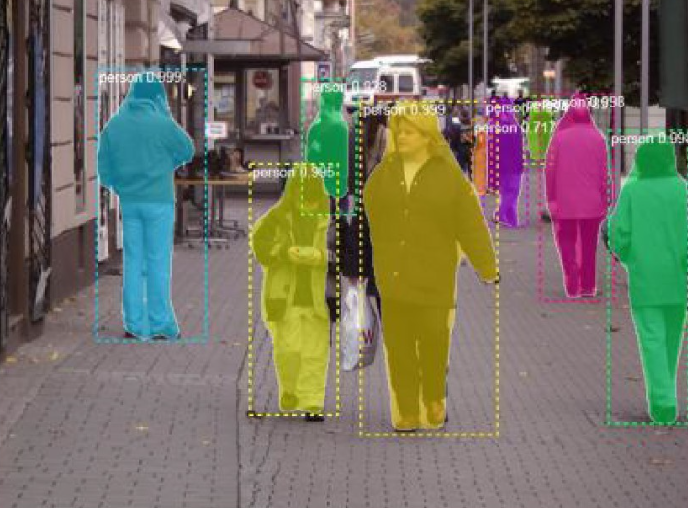
\includegraphics[width=0.85\textwidth]{figures/chapter01/MaskR-CNN物体识别分割结果示例.png}
  \caption{Mask R-CNN物体识别分割结果示例}
  \label{fig:MaskRCNN识别分割示例}
\end{figure}

2019年，王帅等人针对泊车机器人和智能停车库研究领域中对视觉系统的需求，设计了一种基于双目视觉的泊车智能机器车障碍物检测系统。该系统采用物理学中的控制变量法完成双目相机标定，并采用Bouguet算法进行立体校正，引入YOLO卷积神经网络对障碍进行快速检测以确定立体匹配区域，再计算最大视差。实验结果表明，该系统检测平均耗时为0.463s，在1400 mm至2100mm范围内检测误差在50mm内，具有良好的实时性和较高精度。

\begin{figure}[!htbp]
  \centering
  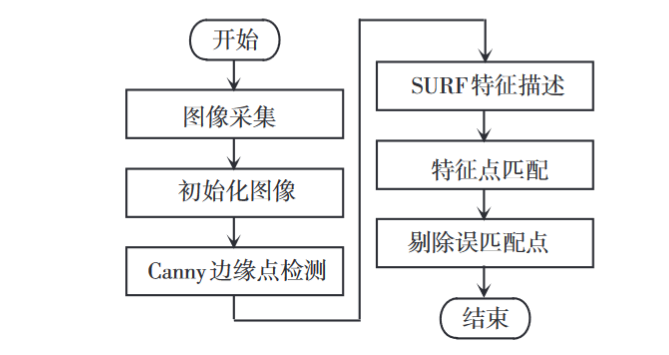
\includegraphics[width=0.85\textwidth]{figures/chapter01/改进立体匹配算法流程图.png}
  \caption{改进立体匹配算法流程图}
  \label{fig:改进立体匹配算法流程图}
\end{figure}

2020年，Xiangmo Zhao和Huayue Wu等人提出了一种基于深度相机的全方位障碍物检测方法，通过在车身周围安装深度相机获取障碍物信息。研究中提出了一种区域生长算法和快速修复方法来提取和修复深度图像中的障碍物区域，并采用改进的迭代归一化切割方法对碎片化和不规则障碍物区域进行聚类和分割，以生成完整的障碍物区域。最终，通过三维可视化方法对障碍物区域进行概览，实现全方位障碍物观察。实验结果表明，该方法在日间和夜间不同环境下对复杂障碍物的检测能力有显著提升，检测速度更快，且不受环境光照影响，从而显著提高了无人驾驶或其他类型车辆的驾驶安全性。

2020年，寇展开和吴健发等人提出了一种无人机障碍物实时感知方法，该方法融合了深度学习、目标跟踪和双目立体视觉技术。首先，通过深度学习对单目相机图像进行障碍物检测与识别，并利用目标跟踪算法实时跟踪障碍物。同时，双目立体视觉技术用于三维重构环境，获取空间信息。通过信息融合策略，准确识别障碍物的种类、位置和大小。实验验证表明，该方法使无人机在搭载双目相机的情况下，能够有效实现障碍物的实时感知。

\begin{figure}[!htbp]
  \centering
  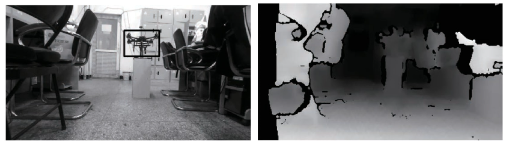
\includegraphics[width=0.85\textwidth]{figures/chapter01/寇展开实现的无人机障碍物实时感知效果.png}
  \caption{寇展开实现的无人机障碍物实时感知效果}
  \label{fig:寇展开无人机障碍物实时感知}
\end{figure}

2021年，魏建胜和潘树国等人设计了一套基于双目视觉的农业车辆障碍物感知系统。该系统使用深度卷积神经网络对作业环境中的障碍进行识别，并提出一种基于改进YOLOv3的深度估计方法。动态场景下系统对障碍物深度估计的平均误差比为4.66\%，平均耗时0.573s，研究结果可为农业机械的自主导航提供有效的环境感知依据。

2021年，Liu Siyao等人开发了一种果园车辆的三目视觉系统，该系统通过结合广角相机和双目立体视觉，实现了果园行间导航和障碍物检测。在图像处理方面，研究设计了基于灰度形态学滤波的树干区域增强算法和光流法的树干区域预测算法，以及基于H通道和G通道图像特性的背景均衡化和干扰削弱算法，以提高检测的准确性和速度。实验结果表明，该视觉系统在0.5m/s和1.0m/s的速度下进行行间检测的平均偏差分别为4.76cm和7.05cm，障碍物距离检测在Z轴方向的平均偏差为3.18cm，在X轴方向为0.45cm，显示出良好的适应性和准确性。

2022年，王峥和赵晓等人针对智能车间中物料位置和运动状态的不确定性，提出一种基于双目视觉的自动导引车(AGV)障碍物检测与避障方法。在障碍物检测过程中，首先采用基于深度检测的障碍物判定算法判断障碍物是否存在：然后利用侦差法提出一种障碍物信息的获取算法，分别得出静、动态障碍物的方位与速度信息。为进一步提高障碍物检测的可靠性，分别对不同状态的障碍物进行检测实验，结果表明，该算法误差较小、结果可靠。

2023年，CAI L和ZHOU C 针对实际道路场景中复杂环境条件，如强光、夜间、雨雪等，提出了一种基于改进YOLOv5算法和双目立体匹配的杆状障碍物检测方法。改进的YOLOv5用于检测和分类杆状障碍物，然后结合双目视觉获取更精确的距离信息。实验结果显示，该方法在杆状障碍物检测上达到了97.4\%的平均精度均值（mAP），比原模型高出3.1\%，图像推理时间仅为1.6毫秒，比原算法快1.8毫秒，模型大小控制在19.0MB以内。此外，系统在3-15米范围内的距离误差小于7\%。综上，该算法实现了实时、准确的识别分类，并确保了特定范围内的精确测量，模型轻量，适合部署在感知系统中。

\begin{figure}[!htbp]
  \centering
  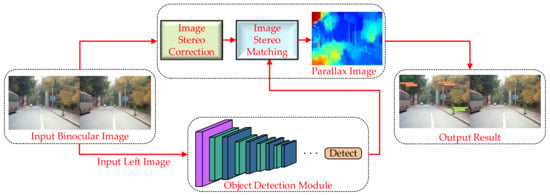
\includegraphics[width=0.85\textwidth]{figures/chapter01/杆状障碍物检测方法.jpeg}
  \caption{杆状障碍物检测方法}
  \label{fig:杆状障碍物检测方法}
\end{figure}

2023年，陈成坤和陈军研针对自动驾驶车辆的障碍物检测与定位问题，提出了一种基于双目视觉和YOLOv4算法的解决方案。该系统利用Jetson Xavier NX硬件平台，通过ZED双目相机获取图像和深度信息，实现了对果园中行人及果树障碍物的实时检测与定位。实验结果表明，系统在准确率和召回率方面表现出色，分别为92.15\%和89.34\%，且在障碍物深度距离方向的平均相对误差控制在1.75\%，显示出较高的定位精度。其检测流程如图~\ref{fig:双目视觉障碍物检测原理图}所示。

\begin{figure}[!htbp]
  \centering
  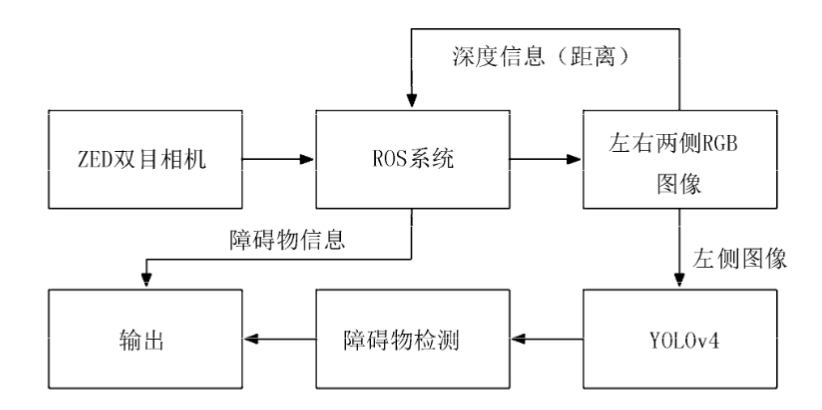
\includegraphics[width=0.85\textwidth]{figures/chapter01/双目视觉障碍物检测原理图.png}
  \caption{双目视觉障碍物检测原理图}
  \label{fig:双目视觉障碍物检测原理图}
\end{figure}

2024年，陈泉淦和陈新元等人针对机耕船自动驾驶功能的需求，设计并实现了一套融合YOLOv5算法和SGBM（半全局匹配）算法的机器视觉障碍感知系统。该系统首先通过收集水田中的人、机耕船和农具等障碍物的图像数据，训练YOLOv5网络模型以获得最优权重，然后在测试中比较了YOLOv5、YOLOv4和Faster R-CNN三种模型的性能。结果表明，YOLOv5在平均精度均值（AP）、检测速度和模型大小方面均优于YOLOv4和Faster R-CNN。特别是在检测机耕船、人和农具时，YOLOv5的置信度分别达到了0.91、0.99和0.95，显示出较高的准确性。

\begin{figure}[!htbp]
  \centering
  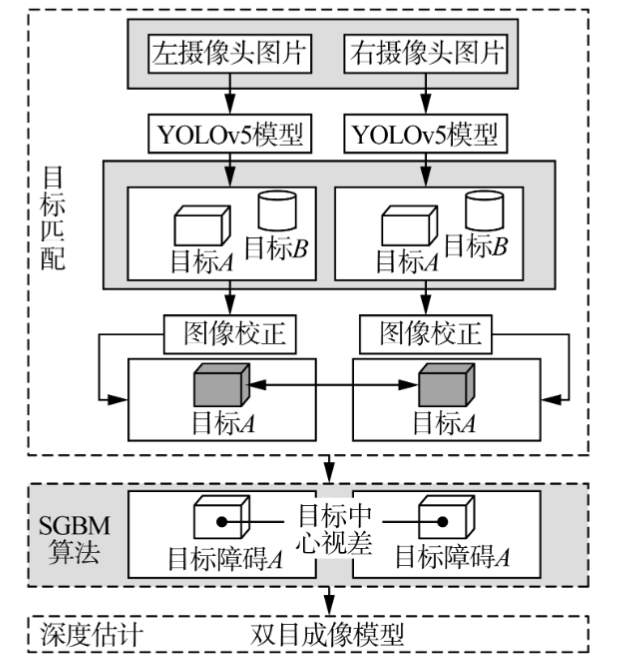
\includegraphics[width=0.45\textwidth]{figures/chapter01/YOLOv5+SGBM测距流程.png}
  \caption{YOLOv5+SGBM测距流程}
  \label{fig:YOLOv5SGBM测距流程}
\end{figure}

\subsection{国内外研究现状综述}

对于两轮平衡车结构的研究主要分为Segway式两轮平衡车、力矩控制的倒立摆平衡车以及变重心式平衡车。Segway式两轮平衡车通过车轮电机控制通过调整车轮转速来实现车体倾斜的调整以维持平衡，有较为成熟的研究基础，该结构广泛应用于平衡车和智能代步车等日常交通工具，但其平衡依赖于车体移动，限制了在静态需求场景下的应用，且在遇到较大外部扭矩或冲击时，电机的调整能力有限；CMG控制则利用飞轮的高速自转和角动量变化来产生控制力矩以调整车体姿态，与车轮电机控制不同CMG能够在车体静止状态下维持平衡，在面对外部冲击时也能够迅速调整车体姿态。然而CMG需要及时控制飞轮进动角回到零位，防止其超出进动幅度造成系统失稳，连续性不如电机控制，且CMG系统的能耗较高，可能影响其在长时间运行中的经济性。现有的两轮平衡车结构虽有一定成果，但各有局限。探索组合式结构，结合不同优势或引入新控制方法，可能为提升性能、增强稳定性和拓展应用场景提供新的突破方向。

关于双目视觉的障碍物感知的研究根据感知方法的不同，双目视觉感知可以分为逻辑方法和深度学习方法；从感知阶段的角度，又可以分为两种主要的处理流程：先进行感知识别再立体匹配和先立体匹配再感知识别。对于不同的实现流程：先识别后匹配流程先对单个摄像头用边缘检测或YOLOv5等模型进行物体识别，再获取深度信息，但深度不参与感知识别过程，易在无特征场景下失效，存在安全隐患。先匹配后感知识别先流程生成视差图，再进行物体感知，能充分利用深度信息，提升感知精度，但计算量大，在低成本平台性能较差。对于感知识别方式：逻辑方法计算需求低、解释性强，但鲁棒性差，感知能力有限。深度学习方法精度高、适应性强，能应对复杂环境，但计算量大，需大量数据支持，嵌入式平台难以实时处理。研究方向应在两者之间平衡，优化嵌入式系统中的实时性和精度。随着科技的进步、设备性能的提升以及深度学习的快速发展，越来越多的研究开始倾向于采用深度学习的方法来进行双目视觉感知。在这一趋势下，"先立体匹配后感知识别"的流程受到广泛关注，因为它能够充分利用深度信息，提升感知精度与鲁棒性，特别是在复杂环境中表现更为出色。



\section{本文主要研究内容及技术路线}

随着智能化技术的发展，城市公园、景区及社区等封闭场景对休闲代步工具的需求日益增加，人们对一种兼顾安全性、舒适性、灵活性及一定趣味性的交通工具需求尤为突出。两轮平衡车因结构紧凑、操控灵活，相较于阿克曼转向结构车辆在狭窄道路更易于转向和倒车操作，成为公园中代步工具的理想选择；考虑到此类场所空间范围较大，对随时召唤的功能需求迫切，平衡车还需能够根据用户指令自主导航至指定位置，从而实现高效、便捷的智能调度服务。

本课题通过功能需求分析，进行载人两轮平衡车的总体设计；根据具体指标设计机械结构和控制系统；根据公园环境感知的需求进行基于双目视觉的感知技术研究；针对实现自动行驶的需求设计自主导航系统；进行实验验证双轮平衡车的基本运动性能、环境感知能力及自动行驶能力的综合表现。具体研究内容如下：

（1）两轮平衡车结构设计与控制系统研究

根据功能需求和具体指标分析，对两轮平衡车进行总体设计，包含对两轮平衡车的机械结构设计和校核，以及电机和传感器的选型和布局；然后基于单片机开发控制系统。

\begin{itemize}
  \item 两轮平衡车的总体设计
  \item 两轮平衡车机械结构的设计
  \item 两轮平衡车控制系统的设计
\end{itemize}

（2）基于双目视觉的感知技术研究

根据环境感知的需求，研究基于深度学习的立体匹配算法，在保证处理速度的前提下获取符合精度要求的视差图；研究基于深度学习的目标检测算法，制作专用数据集并实现对障碍物目标的精准检测；设计算法将深度信息与目标检测结果结合，实现对目标的空间定位，从而完成对环境的有效感知。

\begin{itemize}
  \item 基于深度学习的立体匹配算法的研究
  \item 基于深度学习的目标检测算法的研究
  \item 基于双目视觉的目标空间定位算法的研究
\end{itemize}

（3）两轮平衡车自主导航系统开发

两轮平衡车自动行驶的实现依赖于自主导航系统，该系统主要包括融合定位、环境感知与路径规划等功能模块。在接收到目的地信息后，系统结合定位数据和环境感知结果，规划出合适的行驶路线，并能将运动指令生成相应的运动指令，发送至控制系统，从而实现自动行驶。

\begin{itemize}
  \item 两轮平衡车自主导航系统的设计
  \item 两轮平衡车自主导航系统的硬件环境搭建
  \item 两轮平衡车自主导航系统的软件开发
\end{itemize}

（4）两轮平衡车的实验研究

对两轮平衡车系统的整体性能进行实验验证。测试两轮平衡车在不同路面条件和控制指令下的基本行驶性能，评估其稳定性和响应能力；对双目视觉环境感知算法进行测试，验证目标检测的准确率以及障碍物测距的精度；在实际场景中测试两轮平衡车的自动行驶能力，通过导航路径的执行情况和避障成功率，评估其在真实环境中的自动行驶性能。

\begin{itemize}
  \item 两轮平衡车基本行驶性能的测试实验
  \item 双目视觉环境感知算法的测试实验
  \item 两轮平衡车自动行驶能力的测试实验
\end{itemize}


